\documentclass[twocolumn,10pt]{article}
\usepackage{graphicx}
\usepackage{listings}
\usepackage{xcolor}
\usepackage{booktabs}
\usepackage{amsmath,amssymb,amsthm}
\usepackage{url}
\usepackage[margin=1in]{geometry}
\usepackage{hyperref}

\lstset{
  basicstyle=\ttfamily\small,
  breaklines=true,
  frame=single,
  numbers=left,
  numberstyle=\tiny\color{gray},
}

\title{Login with Everything}
\author{Andrew Miller, Xinyuan Sun, Novel Tokens\\
\small Teleport / Flashbots[X] \\
\small \texttt{socrates1024@gmail.com}}
\date{March 2026}

\begin{document}
\maketitle

\begin{abstract}
Tired of boring credentials?
Every website on the internet can be an identity provider if you're determined enough.
Actually all you need is to run a browser in an attested environment.
This is easy enough with confidential compute, or even just Github actions... and a VPN.
As an application, we welcome you to a message board where you can log in with everything
\end{abstract}

%% ============================================================
\section{Introduction}

\begin{figure}[t]
\centering
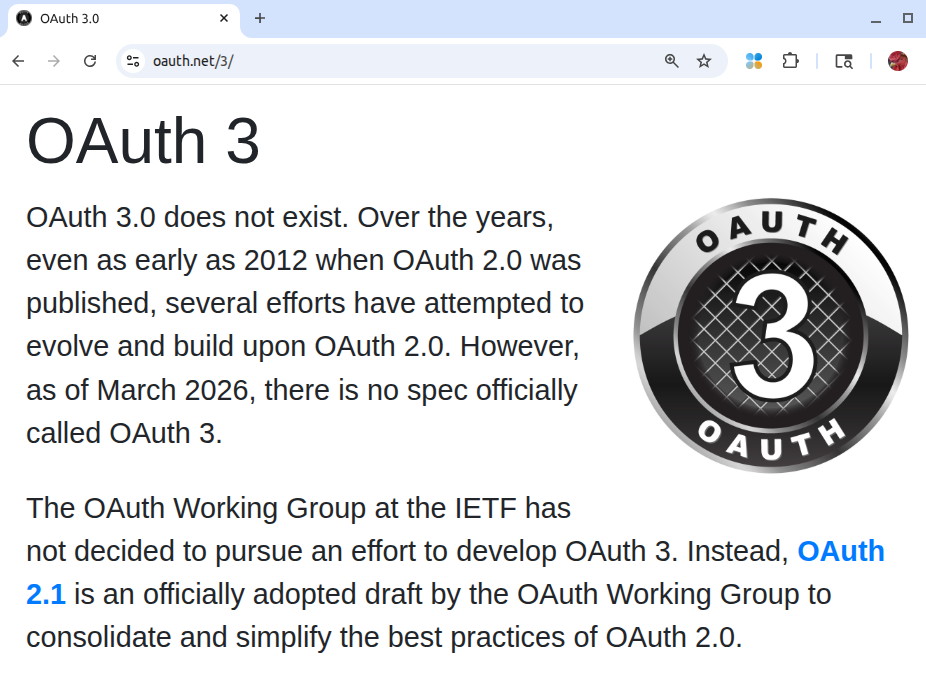
\includegraphics[width=\columnwidth]{oauth3.png}
\caption{OAuth 3 does not exist.~\cite{oauth3}}
\label{fig:oauth3}
\end{figure}

If you want to know whether someone has a GitHub account, why not just... check?
They're logged in. You can see their profile right there. Why do you need OAuth?

This sounds naive.
OAuth exists for good reasons --- the website needs to confirm the user's identity to a third party, cryptographically, without the user just saying ``trust me.''
But notice what OAuth actually does: GitHub runs some code, checks that you're logged in, and signs a token saying so.
The important part is ``checks that you're logged in.''
The signing is just infrastructure.

So: what if you could check that someone is logged in, in a way that produces a signed token, without GitHub's involvement?
You would need two things: their browser session (to see what they see) and a trusted environment (so the check can't be faked).
That's the whole paper.

If this works for GitHub, it works for everything.
Airlines, pharmacies, county tax portals, Neopets.
They're all just websites.
None of them need to build an OAuth endpoint.
None of them need to know they're participating.

\subsection{Related Work}

\textbf{Identity Federation.}
OpenID Connect~\cite{openid-connect}, OAuth 2.0~\cite{rfc6749}.
The assumption that IdPs cooperate.

\textbf{Credential Bridging.}
CanDID~\cite{candid}, DelegaTEE~\cite{delegatee}, SoK: Data Sovereignty~\cite{sok-data}.
Burnt's Redacted File~\cite{burnt-redacted} uses a TDX-based CVM to prove the absence of emails from a specific sender.
Our work: the degenerate case where the credential is ``I'm logged in.''

\textbf{TLS Oracles and zkTLS.}
DECO~\cite{deco}, TLSNotary~\cite{tlsnotary}, Reclaim~\cite{reclaim}, Opacity~\cite{opacity}, ORIGO~\cite{origo}, Janus~\cite{janus}.
TLS oracles prove content of a TLS session.
We prove what a browser shows when logged in --- a strictly easier problem.

\textbf{Anonymous Credentials.}
ASC/U2SSO~\cite{asc}, zk-creds~\cite{zkcreds}, Semaphore~\cite{semaphore}, World ID~\cite{worldid}.

%% ============================================================
\section{Three Problems and a Browser}
\label{sec:how}

\begin{figure*}[t]
\centering
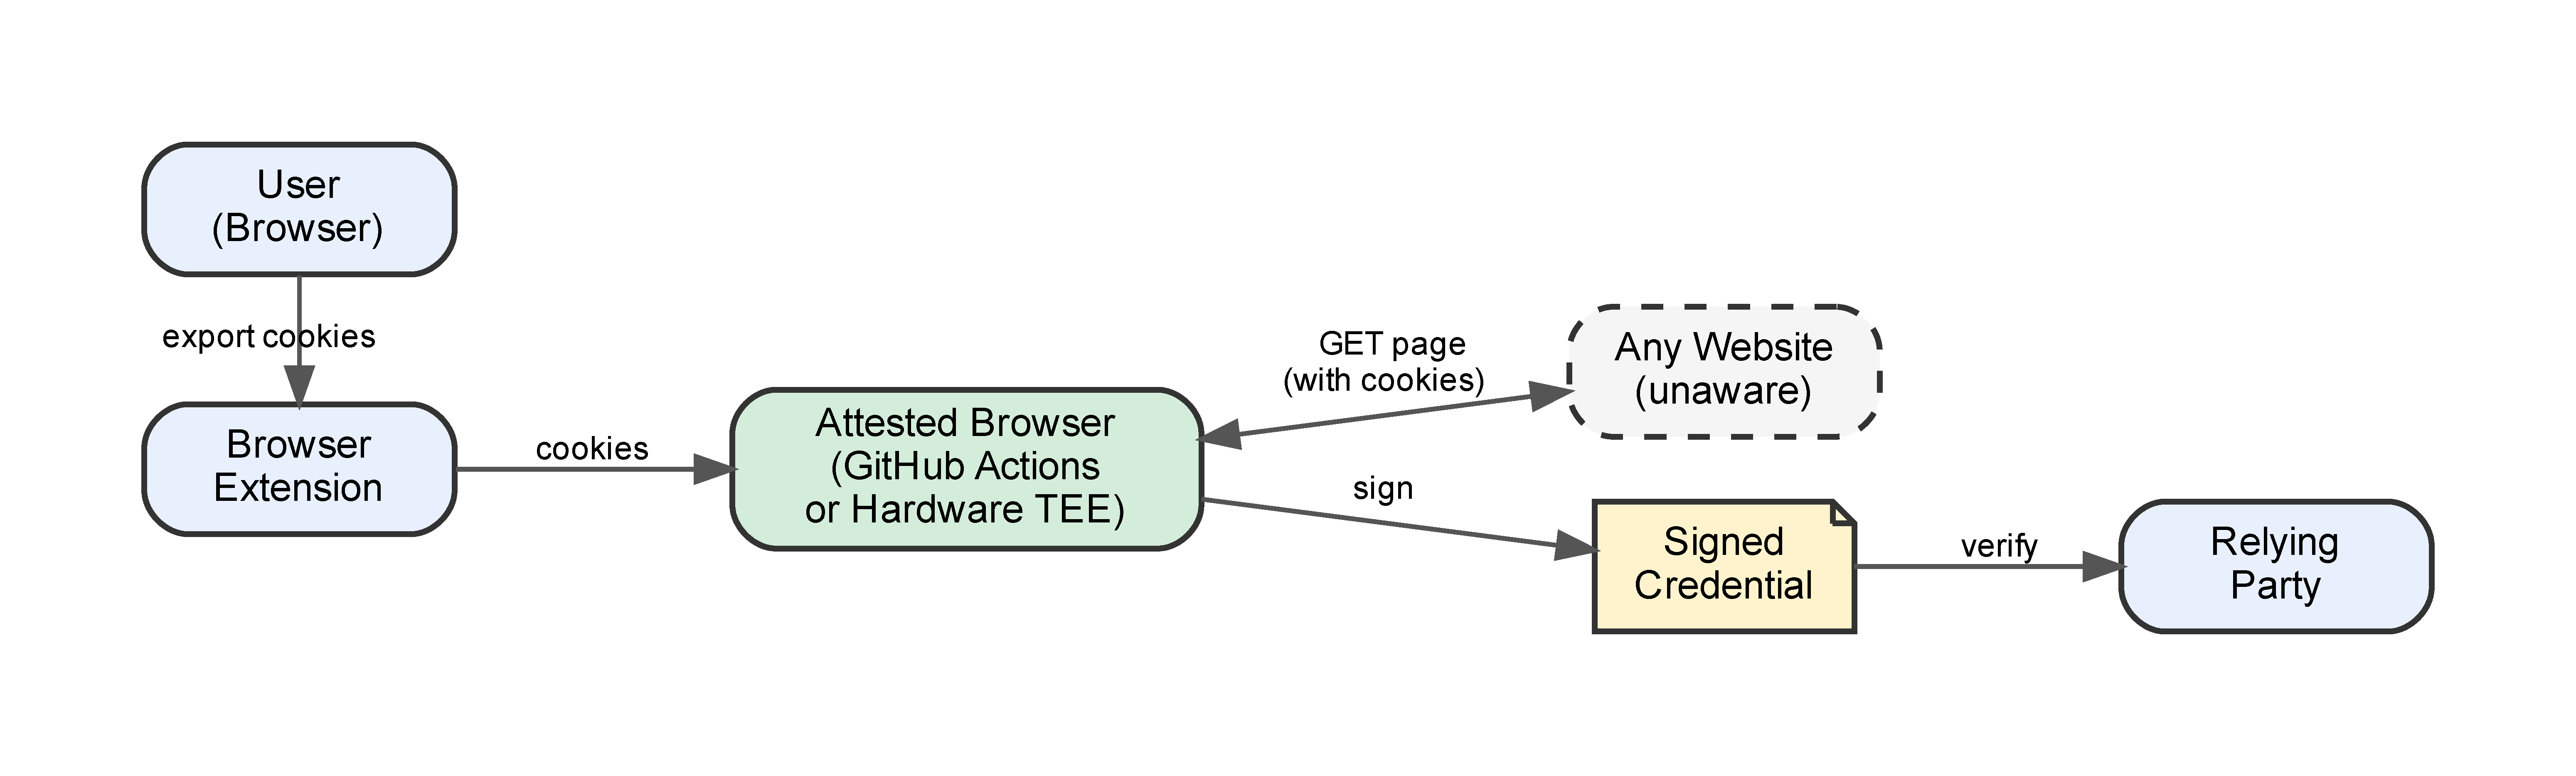
\includegraphics[width=\textwidth]{architecture.pdf}
\caption{System architecture. The user exports cookies via a browser extension. The attested browser logs in, observes the page, and signs a credential. The website is unaware of its role.}
\label{fig:architecture}
\end{figure*}

The plan is: run a browser in a trusted environment, log in as the user, observe the page, sign an attestation.
The website never cooperates and never knows.
This requires solving three problems.

\subsection{Getting the Session}

You can't log into someone's account without their session.
A browser extension exports cookies for a target domain --- the user clicks ``prove,'' picks a site, and the extension packages their session for the attested environment.
This is the only step that touches the user's machine.

\subsection{Trusting the Browser}

Whoever runs the browser controls the output.
If I run it on my laptop, I can make it say anything.
The browser needs to run somewhere I can't tamper with, and the output needs to be signed by that somewhere.

The obvious answer is a hardware TEE --- SGX, SEV, Nitro.
The actual answer, at least for credentials nobody is going to forge, is GitHub Actions.
Each workflow runs in a fresh VM.
Sigstore signs the artifact, binding it to the workflow YAML, commit SHA, and artifact hash~\cite{sigstore, in-toto}.
The workflow file is pinned by commit hash, so auditors can verify the exact code that ran.
This is attestation backed by Microsoft's reputation rather than Intel's silicon, but the threat model is spam bots and sockpuppets, not nation-states.

For high-stakes credentials (financial, medical), the same code runs in a hardware TEE via Dstack~\cite{dstack}.
Only the trust root changes.

\subsection{Handling Every Website}

The browser can visit any URL, but ``check if logged in'' means different things on different sites.
Each site needs an adapter.
The key design decision: make adapters boring.
An adapter defines a \texttt{poll()} function that returns a boolean, passes it to a shared observer that handles the loop, and that's it.

\begin{lstlisting}[caption={GitHub star adapter (actual code).},label=lst:adapter]
import { createObserver } from '../observer.js';

const repo = process.env.REPO;
const ghToken = process.env.GH_TOKEN;

async function poll() {
  const res = await fetch(
    `https://api.github.com/user/starred/${repo}`,
    { headers: {
        'Authorization': `Bearer ${ghToken}`,
        'Accept':
          'application/vnd.github.v3+json',
    }});
  return res.status === 204; // starred
}

createObserver({
  name: 'github-star',
  poll,
  description: `Watching ${repo}`,
}).run();
\end{lstlisting}

For sites we haven't seen before, an LLM generates the adapter: how to detect login state, what's extractable, what's interesting.
The profile gets committed to the repo, pinned by hash, reused for the next user.
Coverage grows with usage.

For interactive liveness --- proving you control an account right now --- the adapter can require observable actions: ``like and unlike this tweet 10 times.''

%% ============================================================
\section{Demo: Login with Everything}
\label{sec:demo}

\subsection{Forum Application}

\begin{figure}[t]
\centering
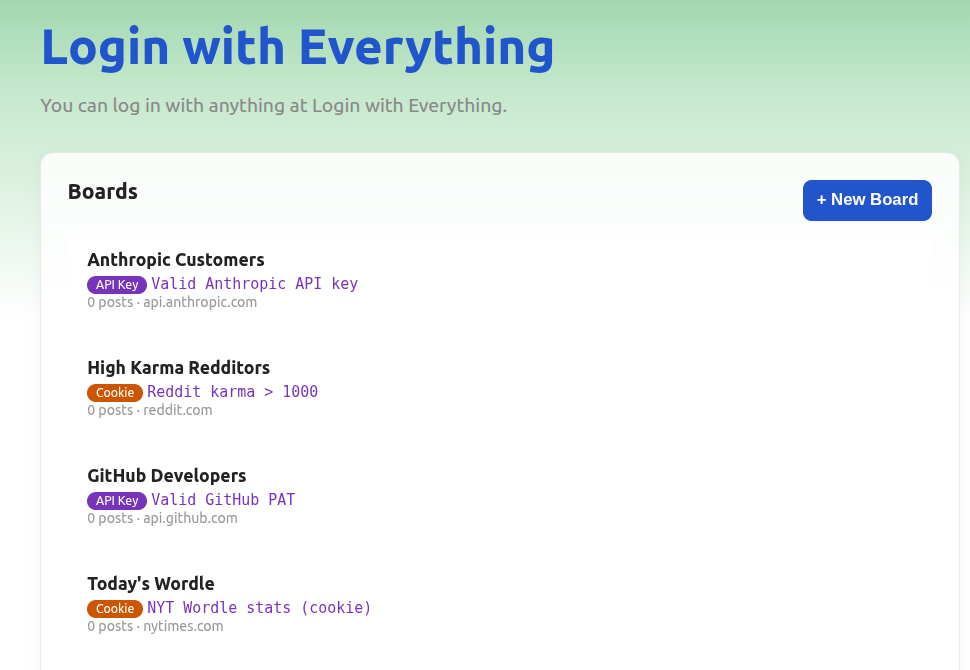
\includegraphics[width=\columnwidth]{forum.png}
\caption{The forum application. Each board defines a login condition: an API key, a cookie-based credential, or a browser session proof. Users who pass the check can view and post.}
\label{fig:forum}
\end{figure}

We built a forum where each board defines its own login condition.
A board creator describes what credential is required --- ``Reddit karma above 1000,'' ``valid Anthropic API key,'' ``NYT Wordle stats via cookie'' --- and an LLM generates the verification plan: which site to check, how to detect login state, and what to extract.

Users who pass the check can view and post to the board.
Users who don't pass see only that the board exists.
Within each board, members are pseudonymous: a nullifier derived from their credential gives them a persistent identity (``same person as last time'') without revealing who they are across boards.

The board itself is the relying party SDK in miniature.
The creator never writes an OAuth integration or a login flow.
They write a sentence describing who should be allowed in, and the infrastructure handles the rest.

%% ============================================================
\section{What to Prove}
\label{sec:longtail}

\textbf{Login with Neopets.}
If your account from 2003 still works, you predate the dead internet.
Your starving Neopet has been waiting.
No LLM would maintain a Neopets account.
More generally, ``login with pre-2022 anything'' is a proof of humanity that gets stronger every year, costs nothing to verify, and is permanently unforgeable.

\textbf{Login with your county tax portal.}
Jurisdictional KYC without showing your address.
Your pharmacy login proves you take medication X for a drug interaction checker without revealing your name.
Your electric utility knows your usage, your address, and whether you own the building.
Carta doesn't need to build an OAuth endpoint for you to prove you hold shares.
These sites have the data already --- they just never agreed to be identity providers, and now they don't have to.

\textbf{Login by logging out.}
To join this forum, prove you deactivated your Twitter account.
Log back in, you're kicked.
Prove you deleted your most popular post --- the TEE confirms your top-performing content no longer exists.
OAuth couldn't express these even if every site cooperated, because the credential is the \textit{absence} of something.

\textbf{Login with quorum.}
N of M people must authenticate within 60 seconds.
The credential is ``I have friends who will do something annoying simultaneously.''
Alternatively: two people must prove opposing positions, one logged into Fox News, the other MSNBC.
Verified disagreement for structured debate.

%% ============================================================
\section{Discussion}
\label{sec:discussion}

\subsection{Nobody Needs a User Table}

The attestation from Section~\ref{sec:how} says ``this person is logged into Neopets.''
That's useful, but it's also linkable --- if you show the same attestation to two different forums, they can collude and figure out you're the same Neopets person.

The fix is standard: wrap the attestation in a zero-knowledge proof.
Register a commitment $c = \mathcal{H}(\texttt{owner\_id} \| s)$ on-chain, prove membership in the set of registered commitments, and output a domain-specific nullifier $\nu = \mathcal{H}(s \| \textit{domain})$.
The nullifier is the same every time you visit the same forum (so they know you're ``that Neopets person again'') but different across forums (so no one can link you).
This is not our contribution --- it's Semaphore~\cite{semaphore}, it's zk-creds~\cite{zkcreds}, it's the standard play.
Our contribution is bootstrapping the master credential from a website that never agreed to participate.

What's new is what this does to the relying party.
If the credential is self-proving, the app doesn't need to verify it against a database.
Which means it doesn't need a database.
Which means it doesn't need a user table, a signup flow, or a password reset page.
The app says ``show me proof you have AAdvantage Platinum'' and either you can or you can't.
There is nothing to store and nothing to delete.
GDPR compliance by construction: you can't leak what you never had.

The most interesting version is continuous.
A group chat called \texttt{\#currently-logged-into-neopets} means exactly what it says.
The TEE re-checks periodically.
You log out of Neopets, you get kicked.
You log back in, you can rejoin.
The channel name is the specification, the enforcement mechanism, and the documentation, all at once.

\subsection{Credentials as Context}

Everything so far uses a credential as a gate: you're in or you're out.
But that's not actually how trust works.
When someone reviews a product, you want to know how many they've bought.
When someone calls a trade, you want to know their exposure.
When someone files a bug report, you want to know if they actually run the software.

The credential doesn't decide whether you can speak.
It decides how seriously to take you.
This is a different thing entirely, and it might be the most useful application of the whole system --- not because it's technically novel, but because it turns out the infrastructure for ``prove you're logged into Neopets'' is the same infrastructure for ``weight this product review by verified purchase history.''
We did not plan this.

%% ============================================================
\section{Security Analysis}
\label{sec:security}

\textbf{Replay.} Attestations are bound to timestamps and run IDs. Relying parties can require fresh runs.

\textbf{Session theft.} If an attacker steals cookies, they can produce fraudulent attestations. This is equivalent to the attacker being logged in --- a pre-existing compromise the protocol does not worsen.

\textbf{Covert channels.} Twitter likes: $\sim$2 bits/second. Amazon cart: much higher bandwidth. The shopping cart as a covert communication channel is left to future work.

%% ============================================================
\section{Conclusion}

The entire concept of ``login'' is a historical accident.
The only reason identity was required was that proving properties required first establishing identity and looking up the property in a database.
Attested browser login inverts this: prove the property directly, skip the identity.

%% ============================================================
\section*{Acknowledgments}

% TODO

\bibliographystyle{plain}
\bibliography{refs}

\end{document}
